\section{Algorithm/Concept}
\label{sec:algorithm}
\graphicspath{{utils/}}
As this Bachelor Thesis tackles two problems, the algorithms can be divided into two categories as well.
The first category consists of racing line recording concepts and the second one of ways to compare these recordings.

\subsection{Recording}
\subsubsection{Visual Odometry}
\label{subsec:vo}
Visual Odometry (VO) is a concept that most camera-based robots use for navigation. It uses two consecutive camera frames to calculate the rotation and translation of the camera between them. The advantage over traditional tracking systems like GPS is, that it isn't dependent on any external sources, like satellites or radio towers, to determine the position of the object.

Also it is capable of much higher polling rates than most GPS receivers, which normally poll at 1 Hz, so they get 1 positional update per second. The potential speed of Visual Odometry is linked to the frame rate of the camera. That way, a camera that records at 30 frames per second enables Visual Odometry to estimate a position 30 times a second. 
The crude algorithm behind VO determines and stores recognizable features in one frame, using a feature detection algorithm and tracks them to a consecutive frame. The displacement of these features determines the direction the camera is traveling.
At first we need two consecutive, rectified camera images. It is important that the images are rectified, because otherwise the edges of the image would be curved and produce wrong results.

Our solution uses the Harris corner detection method for determining features. Finding corners in an image is a very important prerequisite for the final position determination, because it allows us to calculate direction vector to another point. This other point being the same feature in the following camera frame, where the Harris detector is used, as well.\\
These raw data have to be refined for the final step.

One important step for the refinement is outlier removal. External movements, like those of other cars on the track, might cause the algorithm to think the camera was moving when in fact the surroundings moved.
To filter these unwanted movements an iterative method called \textit{Random Sample Consensus} (RANSAC) is used. 
The RANSAC algorithm works by taking a random subset of all the available data, in our case the vectors obtained by the corner detector, and fitting a linear model with a specified neighborhood which contains this subset. All other vectors are then tested against this model and those who fit the model are considered part of the \textit{consensus set}.
If enough vectors lie within this model, it is considered as a viable candidate for a linear approximation. Optionally, the model can be re-evaluated using all vectors in the consensus set.

This sequence of events is repeated a fixed amount of times, each time producing a model which is rejected, because it contains too few inliers, or a refined model, if the model consists of more inliers than the best model so far.

Having two sets of viable corners from either image we can track each feature from one frame to another. 

The Lucas-Kanade method is a way to estimate optical flow from these sets. It observes a local neighborhood around the detected corners and solves the optical flow equation by the least-squares-criterion.

The optical flow equation for a 2D case states that a pixel at position (x, y, t), with t being the time, and intensity $I(x, y, t)$ will have the same intensity after a displacement by $\Delta x, \Delta y$ and $\Delta t$:

\begin{center}
\large
$I(x, y, t) = I(x + \Delta x, y + \Delta y, t + \Delta t)$
\normalsize
\end{center}

Applying the Taylor series, we get:

\begin{center}
\large
$I(x + \Delta x, y + \Delta y, t + \Delta t) = I(x, y, t) + \frac{\delta I}{\delta x}\Delta x + \frac{\delta I}{\delta y}\Delta y + \frac{\delta I}{\delta t}\Delta t$
\normalsize
\end{center}

It follows that: 

\begin{center}
\large
$\frac{\delta I}{\delta x}\Delta x + \frac{\delta I}{\delta y}\Delta y + \frac{\delta I}{\delta t}\Delta t = 0$
\normalsize
\end{center}

or

\begin{center}
\large
$\frac{\delta I}{\delta x}\frac{\Delta x}{\Delta t} + \frac{\delta I}{\delta y}\frac{\Delta y}{\Delta t} + \frac{\delta I}{\delta t}\frac{\Delta t}{\Delta t} = 0$
\normalsize
\end{center}

which results in 

\begin{center}
\large
$\frac{\delta I}{\delta x}\Delta V_x + \frac{\delta I}{\delta y}\Delta V_y + \frac{\delta I}{\delta t} = 0$
\normalsize
\end{center}

where $V_x$ and $V_y$ are the velocity in x and y direction, respectively. $\frac{\delta I}{\delta x}, \frac{\delta I}{\delta y}$ and $\frac{\delta I}{\delta t}$ are the derivatives of the original pixel $(x, y, t)$, which can be written as $I_x, I_y$ and $I_t$.
Thus the optical flow equation turns out to be

\begin{center}
\large
$I_x V_x + I_y V_y = -I_t$
\normalsize
\end{center}

This equation is under-determined, however Lukas-Kanade creates an equation system from all detected points, to determine the optical flow vector $(V_x, V_y)$, that can be written as: 

\begin{center}
\large
$I_x(q_1) V_x + I_y(q_1) V_y = -I_t(q_1)$\\
$I_x(q_2) V_x + I_y(q_2) V_y = -I_t(q_2)$\\
...\\
$I_x(q_n) V_x + I_y(q_n) V_y = -I_t(q_n)$
\normalsize
\end{center}

where $q_1, q_2, ..., q_n$ are the detected corners.

If these equations are written in matrix form Av = b, the result is: 

\[ 
A=
\left[
  \begin{tabular}{cc}
  $I_x(q_1)$ & $I_y(q_1)$ \\
  $I_x(q_2)$ & $I_y(q_2)$ \\
  ... & ... \\
  $I_x(q_n)$ & $I_y(q_n)$ \\
  \end{tabular}
\right],\:
v =
\left[
	\begin{tabular}{c}
	$V_x$\\
	$V_y$
	\end{tabular}
\right],\:
and\: b = 
\left[
	\begin{tabular}{c}
	$-I_t(q_1)$\\
	$-I_t(q_2)$\\
	...\\
	$-I_t(q_n)$\\
	\end{tabular}
\right]
\]

This system is (usually) over-determined. Lucas-Kanade now obtains a solution by minimizing the sum of the squared difference of the results to the determined model.
In that it solves the 2x2 system

	$v = (A^T A)^{-1} A^T b$

Where $A^T$ is the transpose matrix of A.

The final computation is:

\[
\left[
\begin{tabular}{c}
	$V_x$ \\
	$V_y$
\end{tabular}
\right]
= 
\left[
\begin{tabular}{cc}
	$\sum_{i = 1}^n I_x(q_i)^2$ & $\sum_{i = 1}^n I_x(q_i) I_y(q_i)$ \\
	$\sum_{i = 1}^n I_y(q_i) I_x(q_i)$ & $\sum_{i = 1}^n I_y(q_i)^2$
\end{tabular}
\right]
^{-1}
\left[
\begin{tabular}{c}
	$- \sum_{i = 1}^n I_x(q_i) I_t(q_i)$ \\
	$- \sum_{i = 1}^n I_y(q_i) I_t(q_i)$ 
\end{tabular}
\right]
\]

$V_x$ and $V_y$ are now the approximate displacements of every viable corner from one frame to another and can be used to determine the translation and rotation of the vehicle.

If the taken path includes loops it is possible to optimize the result by using loop detection. If any features are re-detected at a later point in time and the current position is close to the position the features were re-detected, the path can be stretched, so that it connects to the earlier path.
This can reduce faulty results that accumulated due to small estimation errors in the previous steps.

\subsubsection{Lane Detection}
Lane Detection uses markings on a road to determine its lateral boundaries in relation to the recording camera. It is often used in autonomous driving and driving assistance systems, because the position of the car in between lane markings gives a lot of information about the direction the car is traveling. 
In our case, not only can we determine a traveling direction, but also the position on the lane.
By tracking the distance to the left and right lane, a deviation to the middle of the lane can be calculated. 
If the driven track is know or the camera is capable of determining a scale (e.g. by using a stereo camera), the deviation can even be expressed as a metric length, which is helpful for extracting additional information, like speed and acceleration, later on.\\
Additionally, not only the racing line can be recorded this way, but also the layout of the track. This is especially useful to determine an ideal racing line later on, because this often requires knowledge of the exact appearance of the race track.

\subsubsection{Recording OBD2 Data}
OBD II (On-board diagnostics 2) is an interface which all cars built after 1996 in the USA or after 2003 in the EU, respectively, have to have built-in. It implements the ELM 327 standard which provides standardized PIDs that return specific car-based sensor data, like the current speed, current motor revolution (rpm), throttle position and more. Connections to the interface are made via a Bluetooth- or USB-adapter.\\
The standard also determines the formatting of the request and return value.\\
The request consists of the required mode and a Parameter ID (PID), which stands for one specific data value. In mode 1 the dongle returns the current values, which is what we need. Other modes, for example, return the values since the last engine failure or information about the car. This request is written to the adapter via a serial port.

\begin{equation}
	\label{eq:obd_example}
		\underbrace{4}_{status code}
		\underbrace{1}_{mode}
		\underbrace{0D}_{PID (hex)}
		\underbrace{37}_{payload}
\end{equation}
\begin{center}
	OBDII example response, returning 55 km/h as the vehicle speed
\end{center}

To make sure that the request arrived correctly, the answer, which will be returned immediately after the request was received, contains some extra data (\ref{eq:obd_example}). The first character is the status. Status 4 means the request was understood and a answer could be delivered. The second, third and fourth characters repeat the obtained request. After that, the payload containing the data is appended. With a formula, which is also specified in the ELM 327 standard, this return sentence can be decoded to an integer number, which represents the real result.

\begin{table}[!ht]
	\begin{center}
		\begin{tabularx}{\textwidth}{|c | X | c | c | c | c | c |}
			\hline
			PID & Size & Description & Min value & Max value & Unit & Formula\\ \hline
			0C & 2 & Engine RPM & 0 & 16 383.75 & rpm & $\frac{256A + B}{4}$\\ \hline
			0D & 1 & Vehicle speed & 0 & 255 & km/h & $A$\\ \hline
		\end{tabularx}
	\end{center}
	\caption{Excerpt of the available OBD II PIDs, A stands for the first, B for the second Byte}
\end{table}

A data request is possible about 10 times per second. This gives us a good basis for further detailed comparisons combined with the racing line recording, as we can determine additional information like acceleration and breaking points, which gear to shift to or at which parts on the track the engine is under especially heavy load, which might be interesting in an endurance race.

\subsection{Comparing}
\subsubsection{Visual Comparison of Racing Line with help of sensor data}
A fairly simple, but effective way to find out where time is lost on the track is the visual comparison of racing lines from different drivers. The idea is to overlay the previously recorded lines over the race track. To actually determine at which point a driver was faster than the other one, we need an obvious optical representation of the speed at any given point on the track and the possibility to receive further information on demand.
In our system, the speed is represented by coloring in the racing line on a gradient scale reaching from green (standing still) to red (>250 km/h).

To do that we use the HSV color space. Due to the circular structure of HSV (see figure \ref{fig:hsv_gradient}), all we need to do normalize the hue part to green (0 km/h) and red (250+ km/h). The color is then simply a function $f(v) = HSV_{hue}$.\\
The HSV value has to then be transfered into RGB color space again.

Besides speed data, different values, like acceleration, braking behavior or lap time, can be displayed in a similar fashion. That way the fastest line for a given corner can be determined and the slower drivers can find out, why their line was inferior.

\begin{figure}[!ht]
\centering
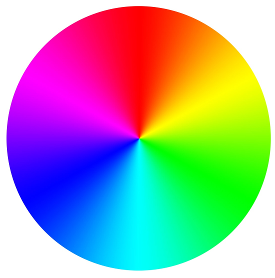
\includegraphics[width=.3\textwidth]{gradient_hsv}
\caption{The Hue portion of the HSV color space}
\label{fig:hsv_gradient}
\end{figure}

\subsubsection{Mathematical Calculation of ideal line given a certain track}
Besides comparing two driver-generated racing lines, it is also possible to calculate a fast, almost ideal racing line.

Bézier curves are a way to depict an entire race track, i.e. a curved path, with a set of control points, \{P\textsubscript{0}, P\textsubscript{1}, ..., P\textsubscript{n}\} (figure \ref{fig:bezier}. In this definition, n is the order of the curve. P\textsubscript{0} and P\textsubscript{n} stand for the beginning and the end point of the curve, respectively, while the intermediate points define the curvature of the curve and don't usually lie on it.

\begin{figure}[!ht]
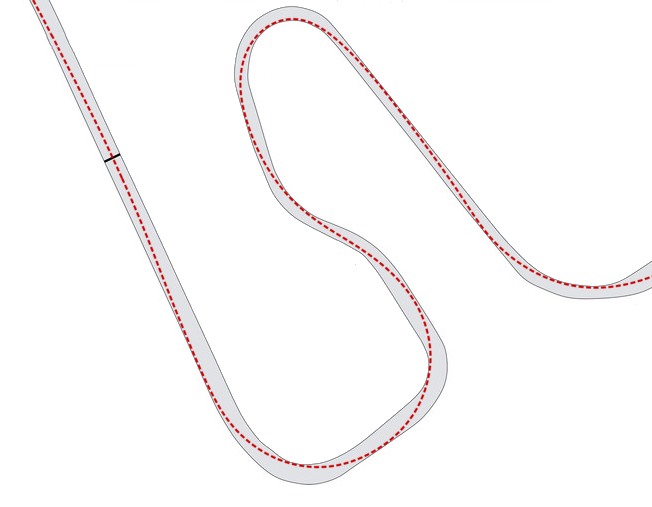
\includegraphics[width=\textwidth]{bezier_track}
\caption{A racing line approximated with a Bézier curve}
\label{fig:bezier}
\end{figure}


As we want to get the line with the least curvature, the Bézier curve is capable of creating a fair approximation, especially suitable for racing beginners.


\subsubsection{Mathematical Comparison of two paths}
To gain additional and more detailed information about the driven racing line, it is helpful to get mathematical values for specific areas (e.g. the entry and exit angle of curves). This can tell a driver that their line was too shallow or too wide and provide the potential to improve.
For this technique we can use either racing line detection algorithm, even GPS. Every pair of consecutive points is turned into a vector, consisting of the distance between the points and the angle $\theta$ to the x-axis (the equator in case of GPS).

\begin{minipage}{\textwidth}
\begin{center}
$\Delta x = endPoint.x - startPoint.x$

$\Delta y = endPoint.y - startPoint.y$

$\overline{xy} = \sqrt{\Delta x² * \Delta y²}$

$\theta = \arctan(\frac{\Delta x}{\Delta y})$ 
\end{center}
\end{minipage}

To speed up subsequent calculations all consecutive vectors with the same $\theta$ can be combined into one vector by generating a new vector with the sum of the magnitude of the old ones. This indicates a straight where the individual sections aren't that interesting.
Now the angle of each section of a corner can be compared. Again, the coloring-approach may be used as a simple way to determine the angle at a glance.
\clearpage
